
\documentclass[12pt]{article}

% Margen de 1 pulgada por lado
\usepackage{fullpage}
% Incluye gráficas
\usepackage{graphicx}
% Packages para matemáticas, por la American Mathematical Society
\usepackage{amssymb}
\usepackage{amsmath}
% Desactivar hyphenation
\usepackage[none]{hyphenat}
% Saltar entre párrafos - sin sangrías
\usepackage{parskip}
% Español y UTF-8
\usepackage[spanish]{babel}
\usepackage[utf8]{inputenc}
% Links en el documento
\usepackage{hyperref}
\usepackage{fancyhdr}
\setlength{\headheight}{15.2pt}
\setlength{\headsep}{5pt}
\pagestyle{fancy}

\newcommand{\N}{\mathbb{N}}
\newcommand{\Exp}[1]{\mathcal{E}_{#1}}
\newcommand{\List}[1]{\mathcal{L}_{#1}}
\newcommand{\EN}{\Exp{\N}}
\newcommand{\LN}{\List{\N}}

\newcommand{\comment}[1]{}
\newcommand{\lb}{\\~\\}
\newcommand{\eop}{_{\square}}
\newcommand{\hsig}{\hat{\sigma}}
\newcommand{\ra}{\rightarrow}
\newcommand{\lra}{\leftrightarrow}

% Cambiar por nombre completo + número de alumno
\newcommand{\alumno}{Diego Iruretagoyena - 14619164}
\newcommand{\todays}{13 de Agosto, 2018}
\rhead{Actividad 0 - \alumno}

\begin{document}
\thispagestyle{empty}
% Membrete
% PUC-ING-DCC-IIC1103
\begin{minipage}{2.3cm}

\includegraphics[width=2cm]{img/logo.pdf}
\vspace{0.5cm} % Altura de la corona del logo, así el texto queda alineado verticalmente con el círculo del logo.
\end{minipage}
\begin{minipage}{\linewidth}
\textsc{\raggedright \footnotesize
Pontificia Universidad Católica de Chile \\
Departamento de Ciencia de la Computación \\
Estructuras de Datos y Algoritmos | IIC2133 \\}
\end{minipage}


% Titul\section*{Introducion }o
\begin{center}
\vspace{0.5cm}
{\huge\bf Actividad 0}\\
\vspace{0.2cm}
\todays\\

\footnotesize{\alumno}
\rule{\textwidth}{0.05mm}
\end{center}

\section*{Introducción}

En el contexto del ramo, hemos estado analizando diferentes estructuras para ordenar informacion. Esto toma vital importancia en los procesos del dia a dia, ya que cada vez estamos generando mas datos, demandando un buen uso y conocimiento de los recipientes en donde los dejaremos.

Para esta actividad hemos implementado un tipo de estructura que utiliza Linked Lists como base. Las Linked List son estructuras que funcionan en base a nodos que tienen referencia a uno o mas nodos contiguos.

Analizaremos seis operaciones clasicas de las Linked Lists, revisando su rendimiento en el tiempo, con numero N arbitrario de informacion, el cual puede ser muy grande. Analizaremos el worst case de cada operacion.


\vspace{0.2cm}
\begin{center}
	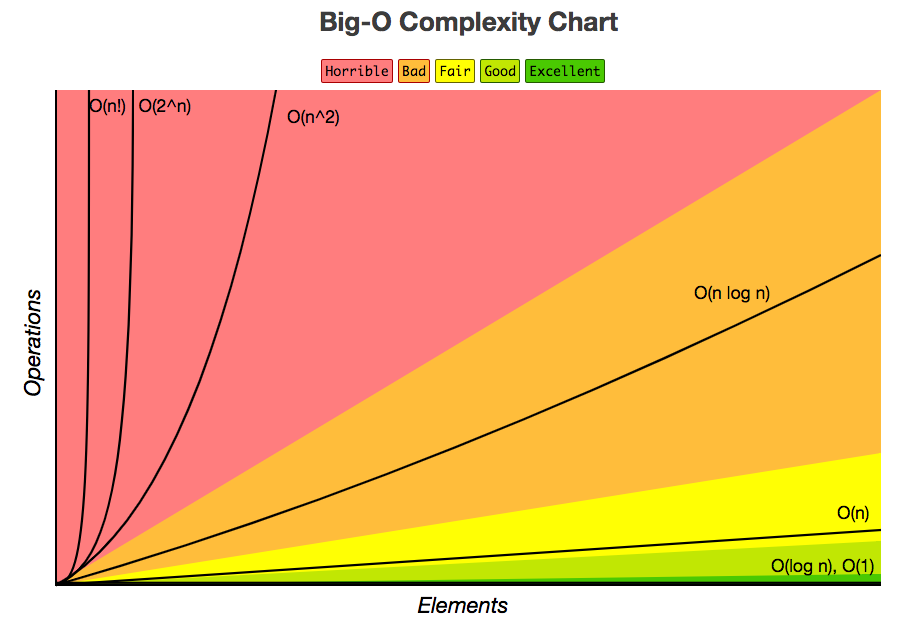
\includegraphics[width=0.5\textwidth]{img/Complex.png}
\end{center}



\section*{Análisis Empírico de Tiempo y Complejidad}

Analizaremos la estructura principal, \textbf{LinkedList}.
Las LinkedList poseen informacion general sobre los nodos que han ingresado. Tiene referencias a su Head y Tail, ademas de posible informacion sobre cuantos elementos tiene. Su unidad basica son los Nodos, quienes tienen un valor y una referencia al Nodo siguiente, en caso de tenerlo (Si no, es NULL). Estos nodos tambien pueden tener referencia a su padre, creando asi una \textbf{Doubly-Linked List}

\subsection*{Complejidad Teorica}
\vspace{0.2cm}

\textbf{1. Insert \\} 
Insertar un elemento es alguna posicion especifica requiere encontrar dicha posicion, actualizar las referencias entre nodos al fijar relaciones nodo parent y next.
Su complejidad es O(n).\\

\textbf{2. Delete \\} 
Al igual que insertar en cierta posicion, eliminar un nodo en la posicion X requiere recorrer elementos hasta dicho valor y luego actualizar las referencias, por lo que su complejidad tambien es de O(n).

\textbf{3. Append \\} 
Como Append busca agregar al final de la lista, podemos hacerlo  ya que tenemos referencia al Head y Tail, por lo que para agregar algo al final, basta con fijar dicho nodo como next de Tail actual, y luego fijarlo como Tail. Su complejidad es O(1).

\textbf{4. Pop \\} 
De forma contraria al append, Pop elimina el ultimo nodo, por lo que aca depende de como construyamos nuestra Linked List. Si es doblemente ligada, basta con ir a Tail, preguntar quien es su parent, fijar dicho nodo como Tail y eliminar el Tail antiguo, lo que podemos hacer facilmente en O(1).\\

\textbf{5. Concatenate \\} 
Al tener referencias de Tail y Head, Concatenate se vuelve O(1), ya que basta conectar las referencias entre el Tail y Head de cada List. Esto lo podemos hacer ya que los nodos son indiferentes a la estructura de las linked list, solo teniendo informacion de su siguiente y posiblemente de su padre, por lo que una vez que conectamos los punteros de referencia, podemos acceder a cualquier parte de la cadena. Una vez que conectamos el Head de Linked List 2 como next de Tail de Linked List 1, y actualizamos Tail Linked List 2 como Tail Linked List 1, obtenemos una Linked List 1 con todos los elementos de ambas estructuras.

\newpage

\textbf{6. Destroy \\} 
Para destruir todos los nodos, debemos ir uno a uno destruyendolo a el y a su next, por lo que la complejidad es de O(n), al tener que pasar por todos los nodos.

\vspace{0.2cm}


\subsection*{Conclusiones}

Como conclusion de esta actividad puedo mencionar el aprendizaje de como la eleccion de la estructura puede incidir fuertemente en los tiempos que demora mi programa. En el curso iremos avanzando en complejidad de estructuras, para luego poder discernir entre las mejores opciones para problemas distintos, ya que no siempre hay una solucion tan clara.

% Fin del documento
\end{document}
